\documentclass[10pt,reqno, final]{ctexart}
%\documentclass{ctexartutf8}
\topmargin=1cm \textwidth=14cm \textheight=21.5cm\oddsidemargin1.2cm\evensidemargin 1.2cm
\usepackage[ bookmarksnumbered, bookmarksopen, colorlinks, citecolor=blue, linkcolor=magenta, unicode]{hyperref}
\usepackage[notcite,notref]{showkeys}

\usepackage{url,hyperref,multirow}
\usepackage{color}
\usepackage{stmaryrd}
\usepackage{exscale}
\usepackage{setspace}
\usepackage{relsize}


\usepackage{epsfig,subfigure,amssymb,amsmath,version}
\usepackage{amssymb,version,graphicx,fancybox,mathrsfs,bm,pifont,booktabs,framed}%,wrapfig}
\usepackage{cases}
\usepackage{epstopdf}

\usepackage{float}
\usepackage{graphicx}
%\usepackage{pythonhighlight}


\renewcommand{\theequation}{\thesection.\arabic{equation}}
\newtheorem{lemma}{引理}[section]
\newtheorem{theorem}{定理}[section]
\newtheorem{corollary}{推论}[section]
\newtheorem{proposition}{性质}[section]
\newtheorem{definition}{定义}[section]
\newtheorem{remark}{注}[section]
\newtheorem{example}{例}[section]

\begin{document}
\title{电磁场理论基础}
\author{张\quad 瑞}
\maketitle
\section{简介}
本文拟从电场与磁场的基本物理定律出发,推导出电磁场的Maxwell方程,再通过Maxwell方程得到电场和磁场在空间中的存在形式,即电磁波,而后研究电磁波在空间中传播的由简单到一般的各种模型。由于传播空间的无界性,在实际使用有限元计算的时候,需要应对无界区域,从而导出人工边界方法和完美匹配层 (PML)方法。

\section{Maxwell 方程的发展与推导及其物理含义}
\subsection{静电场}
\paragraph{$\bullet$ 场强矢量$\bm{E}$}在真空中放置一个点电荷,那么这个电荷会在空间中激发出电场,物理学中使用电场线来刻画电场的方向和大小,电场线从正电荷出发,指向负电荷,这便是场强的方向。而场强的大小是通过穿过单位面积的电场线的条数来定义的,即:
\begin{equation}\label{electricfield}
|\bm{E}|=\frac{N_e}{S},
\end{equation}
而穿过给定面积的曲面的电场线条数又叫做穿过这个曲面的\textbf{电通量},所以电场强度的\textbf{大小}又称为\textbf{电通量密度},见图 \ref{eandcoulumb} 左。
\paragraph{$\bullet$ 库仑力}位于坐标原点的点电荷$q$对位于$\bm{r}$处的试探电荷$Q$的电场力为:
\begin{equation}\label{coulombforce}
\bm{F}(\bm{r}) = \frac{1}{4\pi\varepsilon_0}\frac{Qq\bm{r}}{|\bm{r}|^3}.
\end{equation}
当然,在一般的文献中电荷量为$q$的点电荷在$\bm{r}$处的电场强度的定义是通过单位试探电荷在电场中所受到的库仑力来定义的,即:
\begin{equation}\label{columb}
\bm{E}(\bm{r})=\frac{1}{4\pi\varepsilon_0}\frac{q\bm{r}}{|\bm{r}|^3},
\end{equation}
其中,$\varepsilon_0$ 称为真空中的介电常数,见图 \ref{eandcoulumb} 右。值得注意的是不管有没有试探电荷的存在,点电荷在空间中激发的电场始终存在,只是没有了试探电荷那么库仑力为零。

\begin{figure}[htp]
	\centering
	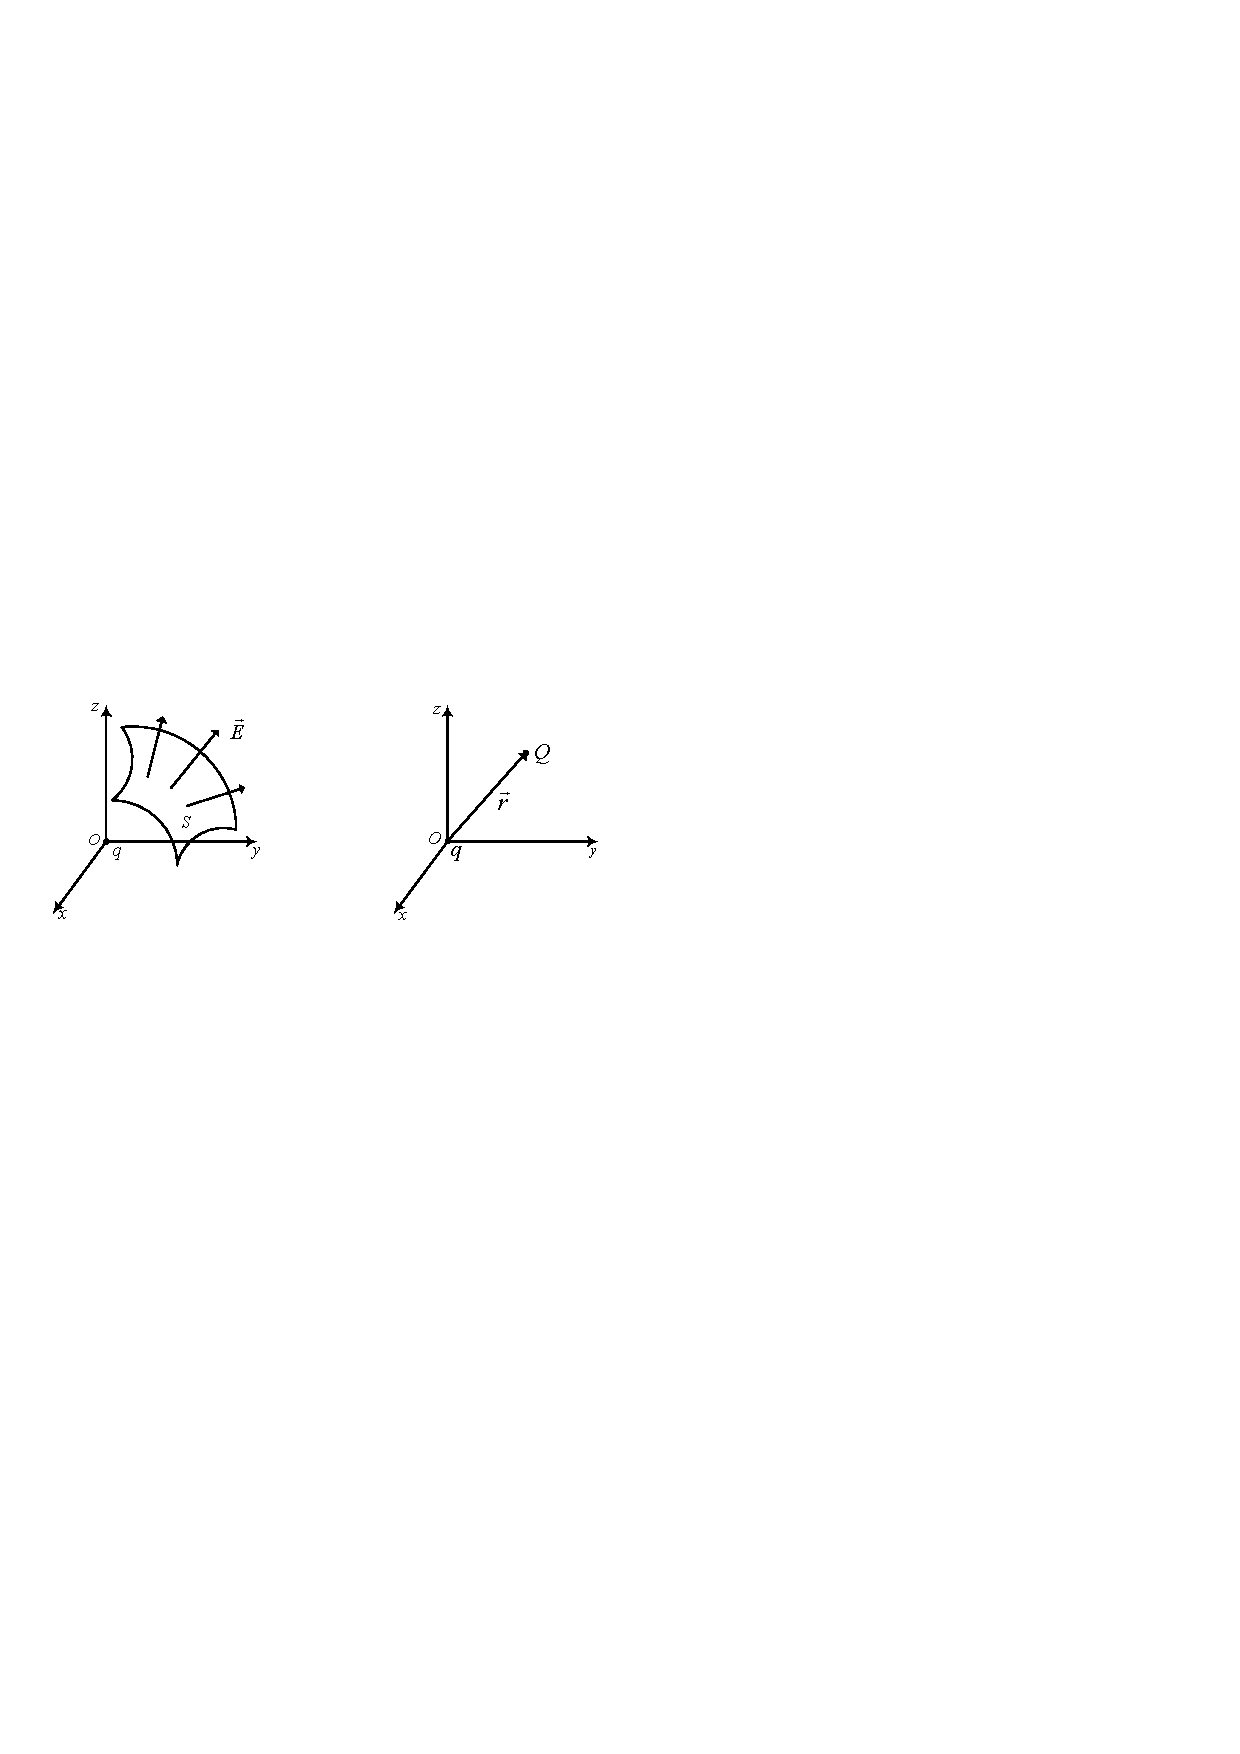
\includegraphics[width=0.8\textwidth]{Figures/EandCoulumb}
	\caption {左:穿过曲面$S$的电通量示意图,右:试探电荷$Q$在$\bm{r}$处所受库仑力示意图. }
	\label{eandcoulumb}
\end{figure}

\paragraph{$\bullet$ 电场在真空中的高斯定律}
设$S$为空间中的一闭合曲面,我们考虑这个闭合曲面的电通量,如图 \ref{gaussthm}左。\textbf{高斯定律} 揭示了闭合曲面的电通量$\Phi_e$, 与该曲面所围成的立体中的电荷总量$\sum q_i$的关系: 
\begin{equation}\label{gaussthm}
\displaystyle \Phi_e = \frac{\sum q_i}{\varepsilon_0} 
\end{equation}

为了计算$\Phi_e$, 我们在闭合曲面上任取一面积微元 $\mathrm{d}S$, 设场强方向与曲面外法向的夹角为$\theta$, 如图 \ref{gaussthm}右,因为场强的大小等于电通量密度,则在$\mathrm{d}S$上的电通量为 
$$E \cos \theta \mathrm{d}S =  \bm{E}\cdot \mathrm{d}\bm{S}$$
于是整个曲面的电通量为
\begin{equation}\label{tongliang}
\Phi_e = \oint_{S}\bm{E}\cdot \mathrm{d}\bm{S},
\end{equation}

进一步,考虑到曲面内的电荷有可能为一般的连续带电体,其电量无法用简单的离散求和来表示,故设曲面内部$\Omega$的电荷体密度为$\rho_e$,  则高斯定律便可写为更一般的形式
\begin{equation}\label{gaussint}
\displaystyle \oint_{S}\bm{E}\cdot \mathrm{d}\bm{S} =\frac{1}{\varepsilon_0} \int_\Omega \rho_e \mathrm{d}\Omega.
\end{equation}

又由向量微积分中的散度定理,我们得到
\begin{equation}\label{gaussdiv}
\int_\Omega \nabla\cdot \bm{E} \mathrm{d}S = \int_\Omega \rho_e\mathrm{d}\Omega,
\end{equation}
由于闭合曲面的任意性,我们得到了真空中电场高斯定律的微分形式:
\begin{equation}\label{gaussthmdiff}
\nabla\cdot \varepsilon_0 \bm{E} = \rho_e.
\end{equation}

\begin{figure}[htp]
	\centering
	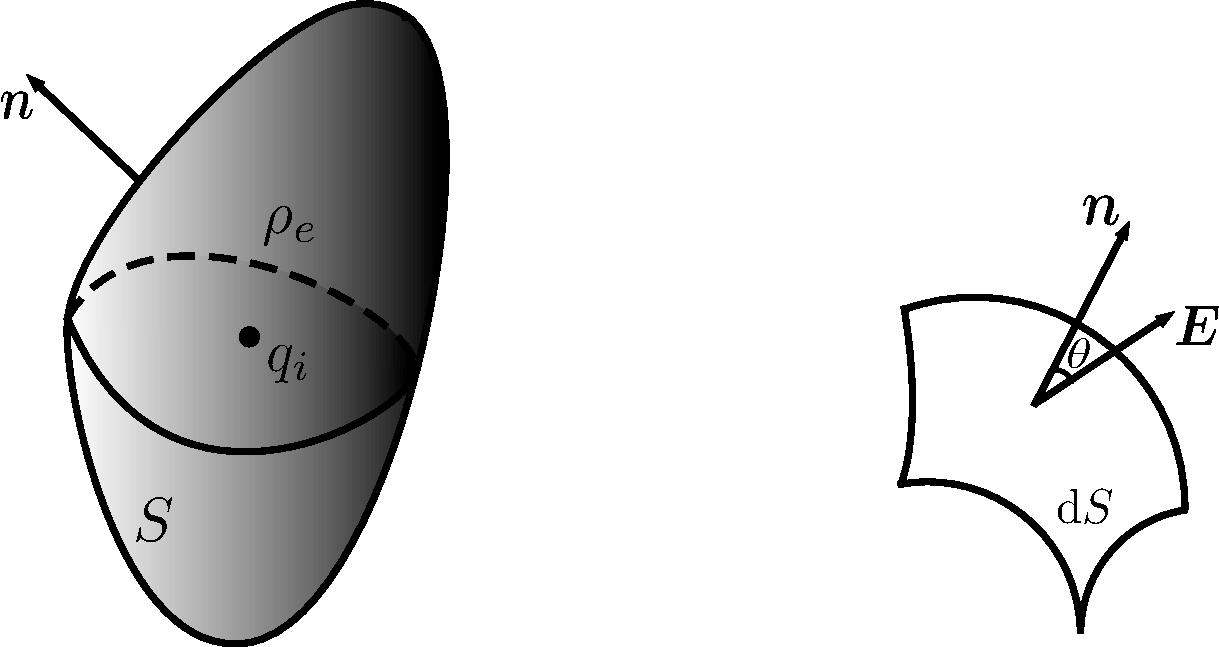
\includegraphics[width=0.6\textwidth]{Figures/GaussThmFig}
	\caption {左:空间中的闭合曲面$S$,右:$\mathrm{d}S$上的电通量示意图. }
	\label{gaussthm}
\end{figure}
\newpage

\paragraph{$\bullet$ 电偶极子} 电偶极子是空间中的一对距离很近电量相等但电性相反的点电荷系统。静电学中使用\textbf{电偶极矩}, 记为$\bm{p}$, 来刻画它们,偶极矩是一个向量,规定其从负电荷指向正电荷,若两个电荷电量的模为$q$, 其距离向量为$\bm{d}$, 则电偶极矩定义为
\begin{equation}\label{dipole}
\bm{p} = q\bm{d}.
\end{equation}

\paragraph{$\bullet$ 电介质的极化现象} 在电场中放置电介质,介质中的分子会发生极化现象,首先由于介质本身并非导体,所以介质内部不会有自由电子在整个介质中运动(像金属),而是由大量的分子构成的,而分子分为极性分子和非极性分子,为了清晰描述极化的过程,我们以非极性分子为例,极性分子的极化虽然较为复杂也稍有不同,但本质机理还是一样的。
\begin{figure}[htp]
	\centering
	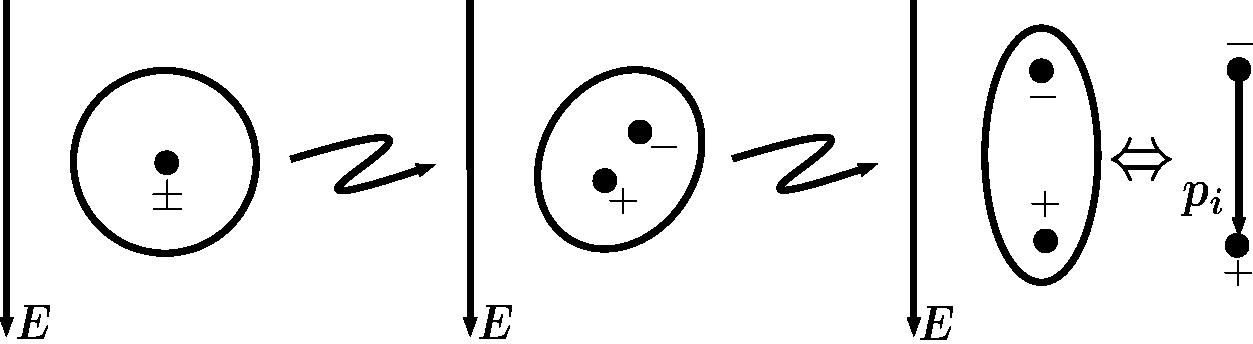
\includegraphics[width=0.6\textwidth]{Figures/polarlization}
	\caption {非极性分子极化过程示意图. }
	\label{polarlization}
\end{figure}

如图 \ref{polarlization} 所示,非极性分子在没有电场的情况下,正负电荷的中心相互重合, 在有了电场之后,由于正电荷与负电荷收到库仑力的作用发生偏移,分子也会在电场中发生旋转,最终形成了一个等效的电偶极子$\bm{p}_i$. 在稳恒电场中,等效的电偶极子的偶极矩与场强方向平行。如此一来,在分子的两端就产生了\textbf{极化电荷},由于极化产生的电荷不是自由电荷,无法自由运动到分子外部,因此有的文献也称为\textbf{束缚电荷}(Bound Charges).
\begin{figure}[htp]
	\centering
	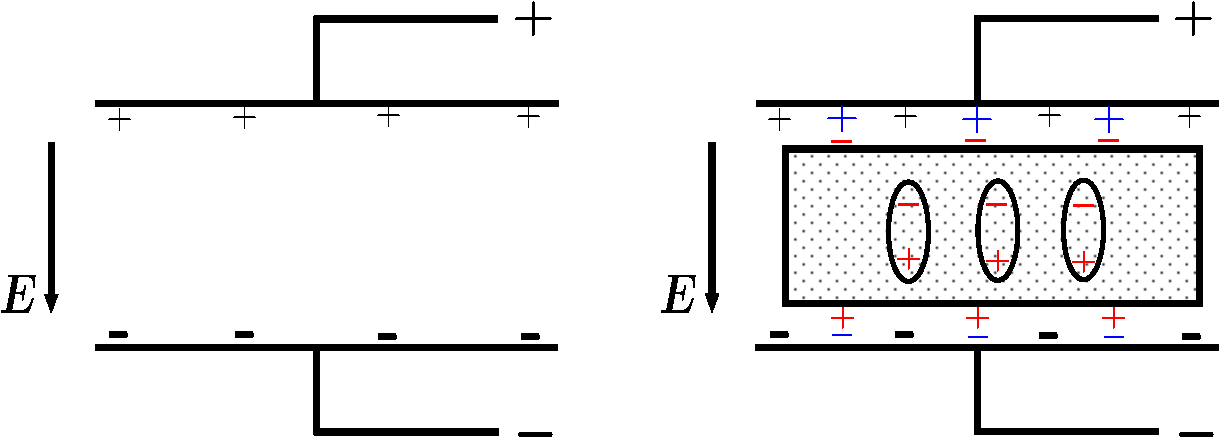
\includegraphics[width=0.6\textwidth]{Figures/jihuashiyan}
	\caption {电介质的极化现象示意图. }
	\label{jihuashiyan}
\end{figure}

现在考虑整个电介质,如图 \ref{jihuashiyan}, 在电介质中每个分子在电场的作用下发生极化现象,于是产生了极化电荷, 显然极化电荷由内部极化电荷和表面极化电荷组成,如图中的介质内部红色标示的电荷与介质表面红色标示的电荷。如果没有介质,在两块电极板上会有一定量的电荷,如图中极板上黑色标示的电荷,一旦放入电介质,由于介质表面产生了极化电荷,而这部分电荷又会在极板上感应出相反的电荷,如图中蓝色标示的电荷,所以加入电介质后极板上的电荷总量反而比原来增加了。

由于每个极化分子都有一个偶极矩,故我们定义一个来刻画电介质受到极化的强度的物理量称为\textbf{电极化密度矢量},记作 $\bm{P}$,它等于单位体积中偶极矩之和,即:
\begin{equation}
\bm{P} = \frac{\sum {\bm{p}_i}}{V}, 
\end{equation}
而当电场稳恒时,每个极化分子的偶极矩与电场方向平行,故整个电极化密度矢量$\bm{P}$也与电场方向平行,且满足:
\begin{equation}\label{P=kappaE}
\bm{P} = \varepsilon_0\chi_e \bm{E}, 
\end{equation}
其中$\chi_e$称为\textbf{电极化率}。
而介质内部的极化电荷与极化密度矢量之间有如下关系:
\begin{equation}\label{innercontribute}
{Q}_{in} = -\int_{\Omega}\nabla \cdot \bm{P}\mathrm{d}\Omega.
\end{equation}

\paragraph{$\bullet$ 电场在介质中的高斯定律} 由于介质内部的电荷量是自由电荷和极化电荷的总和,因此在介质内部的高斯定律需要加上内部极化电荷量$Q_{in}$,即
\begin{equation}\label{jiezhizhong}
\oint_S \bm{E}\cdot \mathrm{d}\bm{S} = \frac{1}{\varepsilon_0}\left[ \int_\Omega \rho_e \mathrm{d}\Omega-\int_\Omega \nabla\cdot\bm{P} \mathrm{d}\Omega \right],
\end{equation} 
由式 	\eqref{P=kappaE}, 与\eqref{innercontribute}, 式	\eqref{jiezhizhong} 可写为
\begin{equation}
\int_{\Omega} \nabla\cdot[(1+\chi_e)\varepsilon_0\bm{E}]\mathrm{d}\Omega = \int_\Omega \rho_e \mathrm{d}\Omega,
\end{equation}
令 
$$\bm{D} = (1+\chi_e)\varepsilon_0\bm{E}:= \varepsilon \bm{E},$$
其中$\varepsilon=(1+\chi_e)\varepsilon_0$称为\textbf{介质中的介电常数}, 而$\varepsilon_r:=1+\chi_e$ 为\textbf{相对介电常数}。
于是我们得到了\textbf{介质中的高斯定律}:
\begin{equation}\label{gaussThmgeneral}
\color{magenta}{\boxed{\nabla\cdot \bm{D} = \rho_e }} 
\end{equation}
显然,通过上述对介质中的介电常数的定义可知,介质中的高斯定律是真空中的推广。

\newpage

\paragraph{$\bullet$ 电场力做功} 在电场中的带电粒子会受到库仑力的作用,这一小节我们来研究电场力对电荷的做功,设电场中带有\textbf{单位电量}的粒子从$A$点沿某一路径运动到$B$点 取线微元 $\mathrm{d}l$, 曲线切方向为$\bm{t}$, 并与场强方向的夹角为$\theta$,如图 \ref{dianchanglizuogong}, 注意到电场强度表达式\eqref{columb},经简单计算可知整个过程库仑力所做的功为
\begin{equation}\label{coulumbwork}
W = \int_{l}\bm{E}\cdot\mathrm{d}\bm{l} = \phi(B) - \phi(A),
\end{equation}
其中$\phi(\bm{r})$称为在$\bm{r}$处的\textbf{电势},满足
$$ \bm{E} = -\nabla\phi, $$
由式\eqref{coulumbwork}可见,\textbf{电场力做功与路径无关,只与粒子始末位置有关},并等于两点的\textbf{电势差}。因此\eqref{coulumbwork}中的积分称为\textbf{路径积分}. 

\begin{figure}[htp]
	\centering
	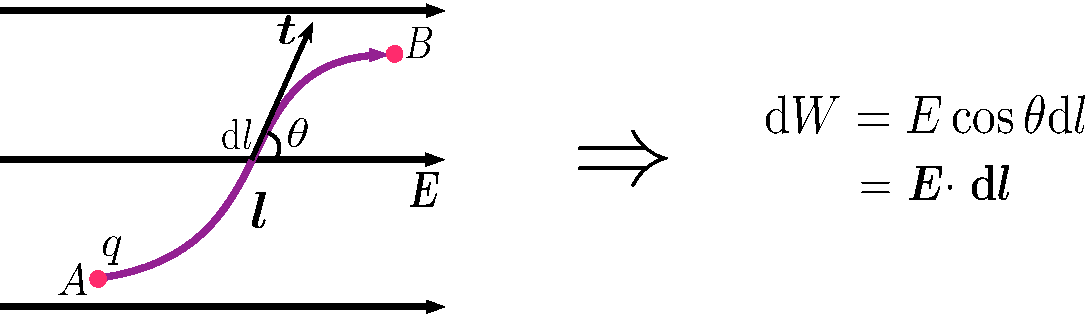
\includegraphics[width=0.6\textwidth]{Figures/dianchanglizuogong}
	\caption {带电粒子在电场中运动示意图. }
	\label{dianchanglizuogong}
\end{figure}

\paragraph{$\bullet$ 真空电场中的环路定理} 本节考虑带电粒子在真空电场中的一种特殊的运动轨迹——封闭的环路, 如图 \ref{dianchanghuanlu}
\begin{figure}[htp]
	\centering
	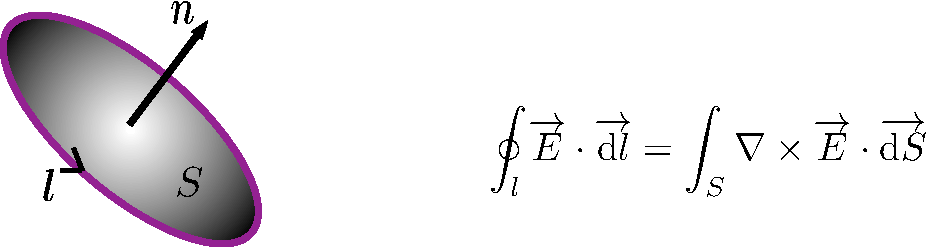
\includegraphics[width=0.6\textwidth]{Figures/dianchanghuanludingli}
	\caption {电场的环路定理示意图. }
	\label{dianchanghuanlu}
\end{figure}

那么由\eqref{coulumbwork}可知只要电场是稳恒的不随时间变化,那么电场力所做的功为零,用数学语言描述就是
\begin{equation}
\oint_l \bm{E}\cdot \mathrm{d}\bm{l} = 0,
\end{equation}
再利用旋度定理,我们得到
\begin{equation}
\int_S \nabla \times \bm{E} \cdot \mathrm{d}\bm{S} = 0,
\end{equation}
于是我们得到了电场的\textbf{环路定理}:
\begin{equation}\label{dianchanghuanludingli}
\color{magenta}\boxed{\nabla\times\bm{E} = 0}
\end{equation}

需要指出的是,即使在空间中存在介质,那么介质内部的环路定理依然是\eqref{dianchanghuanludingli},因为不管在何种介质中,不管电场是否是极化电荷产生的,只要电场力做功,那么做功都只与始末位置有关,与路径无关,所以依然满足式\eqref{dianchanghuanludingli}。

\subsection{静磁场} 上一节介绍了静电场,接下来我们继续介绍静磁场。
\paragraph{$\bullet$ 磁感线} 类似于电场,在真空中放置一块磁铁会在空间中激发\textbf{磁场},磁场也可以使用类似于电场线的\textbf{磁感线}来进行刻画,磁感线从磁铁的$N$极出发指向$S$极,构成一个\textbf{封闭的环线},任意两条磁感线不会相交打结。穿过某个曲面的磁感线条数称为\textbf{磁通量}。

\paragraph{$\bullet$ 磁通量密度矢量 $\bm{B}$} 在电场中场强的刻画使用了电通量密度矢量,类似的,在磁场中为了刻画磁场也定义了\textbf{磁通量密度矢量},国内的教材上通常称为\textbf{磁感应强度},记为$\bm{B}$. 其大小等于穿过单位面积的磁感线条数,即:
\begin{equation}\label{citongmidu}
|\bm{B}| = \frac{N_m}{S}, 
\end{equation}
{\color{blue}{
\fbox{\begin{minipage}{\dimexpr\linewidth-2\fboxsep-2.2pt}
 \paragraph{$\clubsuit$ 电生磁} 在历史上很长一段时间物理学家在研究电场和磁场的时候是各自研究各自的互相不联系,直到安培和奥斯忒做了一个划时代的实验:将一根通电导线靠近一个小磁针,他们发现小磁针发生了微弱的偏转,但只要将导线撤离,那么磁针又回到了平衡位置,重复做该试验发现每次现象都是一样的,由此发现了电能产生磁。从此开始了探寻电与磁之间关系的研究。
\end{minipage}}
}}

\paragraph{$\bullet$ 洛伦兹力} 洛伦兹最先研究了带电粒子在磁场中的受力情况,首先他发现静止的电荷不受力,平行于磁场方向运动的电荷依然不受力,只有当电荷的运动有分量垂直于磁场方向时电荷才受到力的作用,由此得到了\textbf{洛伦兹定律}:磁场中运动的电荷收到磁场力的作用,这个力称为\textbf{洛伦兹力}。设电荷电量为$q$, 则洛伦兹力为:
\begin{equation}
\bm{F} = q\bm{v}\times\bm{B},
\end{equation}
自然地,如果空间中除了磁场还外加了电场,则电荷在电磁场中除了受到磁场力外还受到了库仑力,故合力为
\begin{equation}\label{lorentz}
\bm{F} = q(\bm{E+v\times B}).
\end{equation}
\paragraph{$\bullet$ 磁场与电流的关系—— 毕奥-萨伐尔定律} 洛伦兹研究了带电粒子在磁场中的受力情况,但依然没有解决最初的问题,电流和磁场到底有什么定量的关系?通过实验和理论推导,毕奥和萨伐尔最终得到了通过导线$\bm{l}$的电流$I$和磁场$\bm{B}$的定量关系:
\begin{equation}\label{biotsavertthem}
\displaystyle \bm{B}(\bm{r}) = \frac{\mu_0}{4\pi}\int_l \frac{I\mathrm{d}\bm{l}\times(\bm{r}-\bm{r}^\prime)}{|r-r^\prime|^3}=\frac{\mu_0}{4\pi}\int_l \frac{\bm{J}_e\times(\bm{r}-\bm{r}^\prime)}{|r-r^\prime|^3}\mathrm{d}\bm{r}^\prime, 
\end{equation}
其中,$\mu_0$称为真空中的\textbf{磁导率},$\bm{J}_e$称为\textbf{传导电流密度}。

\paragraph{$\bullet$ 真空中磁场的高斯定律} 类似于电场,这一节我们介绍磁场中的一个重要的定理:\textbf{闭合曲面的磁通量为零}。这个定理称为高斯定律。我们从直观上来理解这个定理,假设空间中有一段通电导线,其电流量为$I$, 则根据毕奥-萨伐尔定律,这个导线在空间中产生了磁通量密度为$B$的磁场其方向满足右手螺旋定则。现在将任意一个闭合曲面$S$放到磁场中,如图 \ref{cichanggaosidingli} 左,那么磁感线便会穿过曲面,如图 \ref{cichanggaosidingli} 右. 

由于磁感线一定是一个封闭的环,那么只要有一条磁感线从曲面的某个位置穿进去,则必定会从另一个地方穿出来,以此才能形成闭合环线,所以所有穿进曲面的磁感线都必定会全部穿出来,则整个闭合曲面的磁通量就为零。

\begin{figure}[htp]
	\centering
	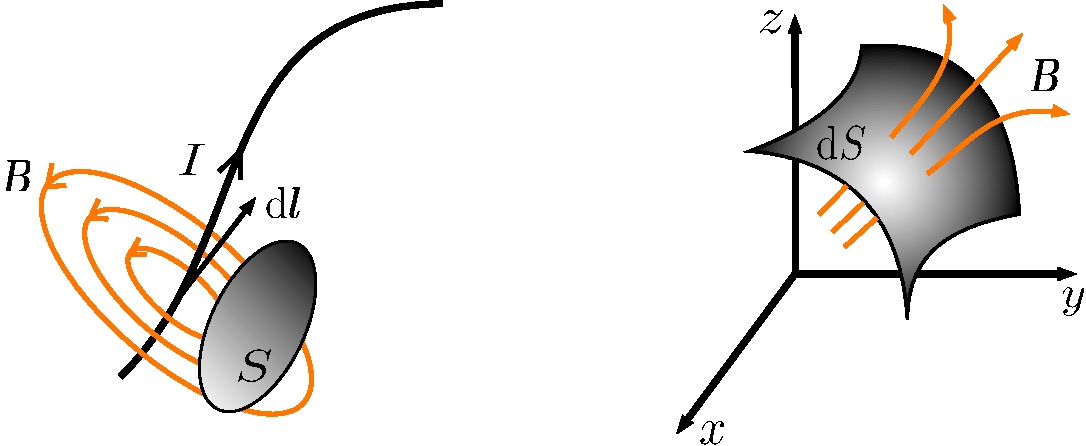
\includegraphics[width=0.8\textwidth]{Figures/cichanggaosidingli}
	\caption {磁场的高斯定律示意图. }
	\label{cichanggaosidingli}
\end{figure}

用公式描述便是:
\begin{equation}
\displaystyle \oint_S \bm{B}\cdot \mathrm{d}\bm{S} = 0,
\end{equation}
又根据散度定理,得到:
\begin{equation}\label{cichanggaosidingli}
\color{magenta}\boxed{\nabla\cdot\bm{B} = 0}
\end{equation}
即使在磁介质中,不管是以何种方式产生磁场,只要是磁感线,就必定是封闭环线,那么介质中的闭合曲面的磁通量依然为零,故在磁介质中的高斯定理依然是式\eqref{cichanggaosidingli}. 

\paragraph{$\bullet$ 真空磁场中的安培环流定理} 在静电场中,电通量密度矢量沿闭合环路的第二类曲线积分为零,在磁场中也有对于磁通量密度沿闭合环路的积分(成为\textbf{环流})的定理,如图 \ref{cichanghuanliudingli}。
\begin{figure}[htp]
	\centering
	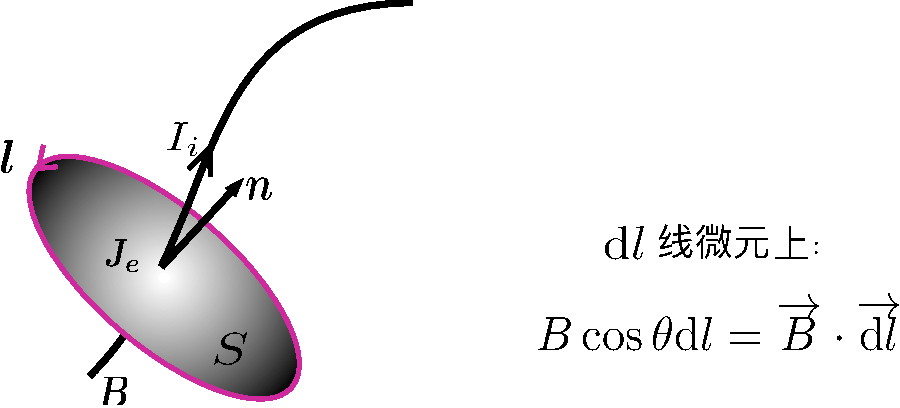
\includegraphics[width=0.6\textwidth]{Figures/cichanghuanliudingli}
	\caption {磁场的安培环流定律示意图. }
	\label{cichanghuanliudingli}
\end{figure}

但与洛伦兹力做功无关,而是与环线所围成的曲面上所有的\textbf{电流}的代数和成正比,这便是著名的安培环流定理:
\begin{equation}\label{huanliu}
\displaystyle  \oint_l \bm{B}\cdot \mathrm{d}\bm{l} =  \mu_0\sum{I_i} = \mu_0\int_S \bm{J}_e \cdot \mathrm{d}\bm{S}.
\end{equation}
其中考虑到面上的电流可能是连续的电流体,其密度就为$\bm{J}_e$, 则总电流便可写成式\eqref{huanliu} 中第二个等号后的面积分。

再由旋度定理可得:
\begin{equation}\label{cichanghuanliudingli}
\color{magenta}\boxed{\nabla\times\frac{\bm{B}}{\mu_0} = \bm{J}_e}
\end{equation}


\paragraph{$\bullet$ 磁介质}









%\section{电磁场的势表示}
%\section{电磁波及其在空间中传播的模型}
%\section{无界区域的处理 —— 吸收人工边界方法}






\end{document}













